\chapter{Jednorozměrná lineární regrese}
Předpokládejme, že sledujeme dvě veličiny $x$ a~$y$, mezi~kterými existuje lineární závislost

 $$
	y = \beta_0 + \beta_1 x,\quad \text{kde } \beta_0, \beta_1 \text{ neznáme.}
 $$

Provede se~experiment a~zjistí se~hodnoty dvojic ($x, y$). Často se~stává, že $x$ je změřeno prakticky zcela přesně.

\begin{remark}
 To nastává například v~případě, kdy se~$x$ nastavuje na~předem dané úrovni a~následně se~k~němu změří odpovídající $y$.
\end{remark}

Oproti tomu u~$y$ obvykle předpokládáme měření s~chybou. Chyba může být náhodná, a~proto i~$y$ budeme chápat jako náhodnou veličinu, kterou budeme značit $Y$.

Pro~dvojice $(x_1, Y_1),...,(x_n, Y_n)$ se~zavádí model

 $$
	Y_i = \beta_0 + \beta_1 x_i + e_i \quad (*) \quad i\in\widehat{n}.
 $$

Jednotlivé proměnné se~pak nazývají následovně

\begin{itemize}
  \item $Y_i$ - vysvětlovaná (závislá) proměnná
  \item $x_i$ - vysvětlující (nezávislá) proměnná, popřípadě \textit{prediktor} nebo \textit{regresor}
  \item $\beta_0,\beta_1$ - neznámé regresní parametry
  \item $e_i$ - náhodný šum, (náhodná chyba)
\end{itemize}

Budeme předpokládat, že $e_i$ jsou nezávislé (někdy bude dokonce stačit, aby byly nekorelované) a~$e_i \sim (0,\sigma^2)$. Z~toho důvodu však splňuje podmínky $\E [e_i] = 0$, $\D [e_i] = \sigma^2$ pro~$\forall i\in\widehat{n}$ (homoskedasticita). Měřením získáme data $(x_1, y_1),...,(x_n, y_n)$ a~cílem statistické analýzy je určit, zda je model ($*$) schopen popsat pozorovanou variabilitu u~$y$.

V \textbf{prvním kroce} odhadneme neznámé parametry $\beta_0, \beta_1, \sigma^2$. Proložíme data přímkou ve~tvaru
 $$
	\widehat{y}(x) = \wbeta_0 + \wbeta_1 x
 $$
a porovnáme pro~$\forall i\in\widehat{n}$ \textbf{naměřená data} $y_i$ s~\textbf{predikovanou hodnotou lineární regrese} $\widehat{y}(x_i)$. To nám umožňuje posoudit adekvátnost modelu.

Pro proložení dat přímkou existuje několik způsobů. Zásadní ovšem bude znalost rozdělení $e_i$ (v~tomto případě i~$Y_i$), i~když apriori není zřejmé, proč znát rozdělení a~nikoliv $\beta_0, \beta_1$.

Máme dvě možnosti,
\begin{enumerate}
  \item odhadnout $\beta_0, \beta_1$ pomocí metody nezávisející na~rozdělení chyb, nebo
  \item udělat věrohodnostní předpoklad o~rozdělení chyb, odhadnout $\beta_0, \beta_1$ a~následně ověřit předpoklad.
\end{enumerate}


\begin{remark}
 Speciální důležitý případ je $e_i \sim \NN(0,\sigma^2)$, který při~MLE odhadu $\beta_0, \beta_1$ vede na~metodu nejmenších čtverců, která může být použita bez~ohledu na~rozdělení chyb.
\end{remark}

\section{Odhady parametrů}
\subsection{Data s~předpokladem normality dat}
Předpokládáme, že $e_1,..., e_n ~iid~\NN(0,\sigma^2)$. To znamená, že $Y_i \sim \NN(\beta_0 + \beta_1 x_i,\sigma^2)$ a~$Y_1,..., Y_n$ jsou nezávislé.

\subsection*{MLE odhady}

Věrohodnostní funkce je ve~tvaru

 $$
\begin{aligned}
	L = L (\beta_0, \beta_1, \sigma^2) = \left(\frac{1}{ \sqrt{ 2 \pi \sigma^2 }} \right)^n \exp \left(- \frac{1}{2 \sigma^2 } \sumin(y_i -  \beta_0  - \beta_1 x_i)^2 \right), \\
l = \ln L = -\frac{n}{2} \ln (2 \pi) -\frac{n}{2} \ln (\sigma^2) - \frac{1}{2 \sigma^2 } \sumin(y_i -  \beta_0  - \beta_1 x_i)^2.
\end{aligned}
 $$

Pro pevné $\sigma^2 > 0$ je maximalizace $l$ ekvivalentní s~minimalizováním $S$, kde

 $$
S = S(\beta_0, \beta_1) = \sumin(y_i -  \beta_0  - \beta_1 x_i)^2.
 $$

Proto tuto metodu někdy nazýváme metodou nejmenších čtverců.

 $$
\begin{aligned}
&\frac{\partial S}{\partial \beta_0} = - 2 \sumin(y_i -  \beta_0  - \beta_1 x_i) = 0, \\
&\frac{\partial S}{\partial \beta_1} = - 2 \sumin(y_i -  \beta_0  - \beta_1 x_i) x_i = \sumin y_i x_i - \beta_0 \sumin x_i - \beta_1 \sumin x_i^2 = 0.
\end{aligned}
 $$
Z první rovnice pak dostaneme
 $$
 \beta_0 = \frac{1}{n} \sumin y_i -  \beta_1 \frac{1}{n} \sumin x_i = \overline{y}_n - \beta_1 \overline{x}_n
 $$
a dosazením do~druhé dostaneme výraz
 $$
\sumin y_i x_i - \overline{y}_n \sumin x_i - \beta_1 \overline{x}_n \sumin x_i - \beta_1 \sumin x_i^2 = 0.
 $$
Jednotlivé MLE odhady parametrů pak mají následující tvar
 $$
\wbeta_0 = \overline{y}_n - \wbeta_1 \overline{x}_n \quad \text{a}~\quad
\wbeta_1 = \frac{\sumin y_i x_i - n \overline{x}_n \overline{y}_n}{\sumin x_i^2 - n \overline{x}_n^2}.
 $$

Nyní najdeme odhad parametru $\sigma^2$

 $$
\frac{ \partial l}{ \partial \sigma^2} = -\frac{n}{2} \cdot \frac{1}{\sigma^2} + \frac{1}{2 (\sigma^2)^2} \sumin (y_i -  \beta_0  - \beta_1 x_i)^2 = 0,
 $$
vyjádřením $\sigma^2$ z~rovnice dostaneme výraz
 $$
\widehat{\sigma}^2 = \frac{1}{n} \sumin (y_i -  \beta_0  - \beta_1 x_i)^2 = \frac{1}{n} \sumin (y_i -  \widehat{y}_i)^2 = \frac{1}{n} \SSE,
 $$
kde $\widehat{y}_i = \beta_0  - \beta_1 x_i$ je predikce modelu (odhad $\E [Y_i]$) a~zkratka $\SSE$ je odvozena z~anglického \textit{sum of the squares of errors}. Rozdíl $\widehat{e}_i = y_i -  \widehat{y}_i$ nazýváme $i$-té reziduum. Velikost reziduí indikuje, jak dobře odhadnutá přímka odpovídá datům. Rezidua jsou vlastně odhady chyb $e_i$,  jejich analýza hraje významnou roli v~ověření předpokladů rozdělení chyb.

\subsection*{Odhad $\sigma^2$}
Pro odhad $\sigma^2$ se~používá častěji statistika s názvem \textbf{standardní chyba regrese} (\textit{standard error}) ve tvaru $$s^2_n = \frac{1}{n - 2} \sumin (y_i -  \widehat{y}_i)^2 = \frac{1}{n-2} \SSE,$$ která je nestranným odhadem parametru $\sigma^2$ (pro libovolné rozdělení $e_i$), zatímco $\sigma^2_{\text{MLE}}$ je vychýlený odhad i~pro~normální rozdělení chyb.

\subsection{Data bez~předpokladu normality}
V tomto případě jsou tedy $e_1,..., e_n$ nekorelované, $e_1,..., e_n \sim (0,\sigma^2)$.
Pro odhad $\beta_0, \beta_1$ lze použít minimalizaci S~(metodou nejmenších čtverců), což je rozumné provedení, když si uvědomíme geometrickou interpretaci.

Nechť $y = \beta_0 + \beta_1 x$ je rovnice nějaké přímky, potom $y_i - (\beta_0 + \beta_1 x_i)$ je vertikální vzdálenost bodu $(x_i,y_i)$ od~přímky a~
 $$
 S~ = \sumin (y_i - \beta_0 - \beta_1 x_i)^2
 $$
je míra udávající, jak dobře přímka prokládá data. Dává smysl vybrat takovou přímku, která minimalizuje S. Minimalizací S~získáme stejné odhady $\wbeta_0, \wbeta_1$ jako u~MLE odhadů pro~normální data. Teď se~ale nazývají odhad \textbf{metodou nejmenších čtverců} LSE (least squares estimators).
Existuje více měr vhodnosti přímky. Použití LSE pro~libovolné rozdělení chyb má dvě zdůvodnění.
\begin{enumerate}
  \item Pro~normální rozdělení chyby LSE splývá s~MLE.
  \item LSE odhad je navíc BLUE (best linear unbiased estimator), jak ukážeme v~Gauss–Markovově větě.
\end{enumerate}

\begin{example}
Nechť $e_1,..., e_n$ jsou $~iid~$ s~hustotou
\begin{equation*}
  f(\epsilon) = \frac{1}{2} \e{- | \epsilon |} \quad (\text{Laplaceovo rozdělení}).
\end{equation*}
Potom je hustota $Y_i$ rovna
\begin{equation*}
  f_{Y_i}(y_i) = \frac{1}{2} \e{- | y_i - \beta_0 - \beta_1 x_i |}
\end{equation*}
a věrohodnostní funkce $L$ a~$l$ mají tvar
\begin{equation*}
\begin{aligned}
  L & = \frac{1}{2^n} \e{- \sumin | y_i - \beta_0 - \beta_1 x_i |},  \\
  l & = -n \ln 2 - \sumin | y_i - \beta_0 - \beta_1 x_i | .
\end{aligned}
\end{equation*}
MLE odhady parametrů $\beta_0, \beta_1$ získáme minimalizací
 $$
A = \sumin | y_i - \beta_0 - \beta_1 x_i |,
 $$ které nazýváme \textbf{MAD} (\textit{minimum absolute deviation}). Zde budou odhady jiné, než u~LSE.

Uvažujme 3 body: $(0,0),~ (1,0),~ (\frac{1}{2},\frac{1}{2})$.
 $$
\begin{aligned}
&\MLE: \quad  \beta_0 = \beta_1 = 0, \quad A~ = 0.5
, \quad \widehat{y} = 0 \\
 &\LSE: \quad \overline{x} = \frac{1}{2}, \overline{y} = \frac{1}{6}, \quad \sumin x_i^2 = \frac{5}{4}, \sumin x_i y_i = \frac{1}{4}, \quad \beta_1 = 0, \beta_0 = \frac{1}{6}
  \end{aligned}
 $$
\end{example}

\begin{center}

    \begin{tikzpicture}
    \node[inner sep = 0pt] (pic) at (0,0)
    {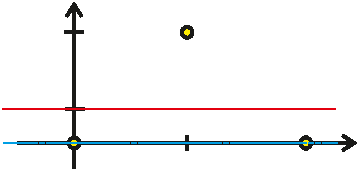
\includegraphics[width = 13cm]{pictures/picture_1_F.pdf}};
    \draw [color = red](4.5,-0.2) node[anchor = north west] {LS line};
    \draw [color = blue](4.5,-1.3) node[anchor = north west] {MAD line};
    \draw [color = black](4.45,-2.5) node[anchor = north west] { $1$ };
    \draw [color = black](-4.5,-2.45) node[anchor = north west] { $0$ };
    \draw [color = black](0,-2.35) node[anchor = north west] { $\frac{1}{2}$ };
    \draw [color = black](-4.55,1.8) node[anchor = north west] { $\frac{1}{2}$ };
    \draw [color = black](-4.55,-1) node[anchor = north west] { $\frac{1}{6}$ };
    \end{tikzpicture}
\end{center}

\begin{remark}
I když $s^2_n$ je nestranný odhad $\sigma^2$, $s_n$ je vychýlený odhad $\sigma$!
Je to obecná vlastnost odhadů (nestranných) rozptylů, neboť pokud je $s^2$ nestranný odhad $\sigma^2$, pak $\E[s] \leq \sigma$.
\end{remark}
\begin{proof}
Uvažujme náhodnou veličinu $X$, pro~kterou platí, že $\D [X] < + \infty$. Po dosazení $X = s$ do známé rovnice $ \E [X^2] = \D [X] +  \E [X]^2$ dostaneme vztah $$\E [s^2] = \D [s] +  \E [s]^2,$$ kde $\E [s]^2 \leq \sigma^2$, $\E [s] \leq \sigma$ a rovnost nastává, pokud $\D [s] = 0$.

\end{proof}
Například pro~normální chyby je $s_n^2 \, \propto \, \chi^2 \Rightarrow \E [s_n] < \sigma$.

\begin{remark}
Předpokládali jsme, že hodnoty $x_i$ jsou dány přesně, což nemusí být vždy pravda. Často jsou obě veličiny $(x,y)$ měřeny nepřesně. Existují EIV models \uv{error in variable}, v~těchto modelech jsou často preferovány jiné odhady než LSE. Populární metoda je dále \textbf{total least squares} (\textit{ortogonal least squares}). Zde minimalizujeme $\sumin d_i^2$, kde $d_i$ je vzdálenost bodu a~přímky (kolmice na~přímku protínající bod). To znamená, že neupřednostňujeme veličinu $x$, ale přistupujeme k~$x$ a~$y$ rovnoměrně.
\end{remark}

\begin{center}
    \begin{tikzpicture}
    \node[inner sep = 0pt] (pic) at (0,0)
    {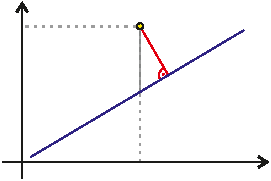
\includegraphics[width = 13cm]{pictures/picture_2_F.pdf}};
    \draw [color = red](1.0,2.3) node[anchor = north west] { $d_i$ };
    \draw [color = red](2.0,1.0) node[anchor = north west] {TLS vzdálenost};
    \draw [color = gray!20!black](-2.6,1.7) node[anchor = north west] {LS vzdálenost};
    \draw [color = red!20!black](0.0,3.80) node[anchor = north west] { $(x_i,y_i)$ };
    \draw [color = black](5.45,-3.65) node[anchor = north west] { $x$ };
    \draw [color = black](0,-3.65) node[anchor = north west] { $x_i$ };
    \draw [color = black](-6.25,3.8) node[anchor = north west] { $y$ };
    \draw [color = black](-6.25,3.3) node[anchor = north west] { $y_i$ };
    \end{tikzpicture}
\end{center}

\begin{remark}
V literatuře se~někdy $x$ uvažují jako realizace náhodné veličiny (ne vždy se~$x$ nastavuje předem, nebo je jasně dané).
\end{remark}
Model má potom tvar
 $$
 \E [Y_i | X_i] = \beta_0 + \beta_1 X_i, \quad  \D [Y_i | X_i] = \sigma^2.
 $$
Pro většinu výsledků prezentovaných v~této přednášce ale není podstatné, zda je $x$ chápáno jako pevné nebo náhodné.
Důkazy většinou fungují s~podmíněnými výrazy $(\E, \D,...)$ při~dané hodnotě $x$ místo~nepodmíněných.
Větší pozornost je naproti tomu potřeba u~odvození asymptotických rozdělení odhadů.

\subsection{Vlastnosti odhadů $\widehat{\beta}_0,~ \widehat{\beta}_1, ~ s_n^2$}
\begin{theorem}
   Nechť $\widehat{\beta}_0, \widehat{\beta}_1$ jsou $\mathrm{LSE}$ odhady parametrů $\beta_0, \beta_1$ v~lineárním modelu
 $$
   		Y_i = \beta_0 + \beta_1 x_i + e_i, \quad i\in\widehat{n},
 $$
   kde $e_i$ jsou nezávislé náhodné veličiny (postačí i~nekorelovanost) se~stejným rozptylem $\sigma^2$. Potom platí, že
   \begin{enumerate}
  \item $\E [\widehat{\beta}_0] = \beta_0, \quad \E [\widehat{\beta}_1] = \beta_1$, (nestranné odhady),
  \item $\D [\widehat{\beta}_1] = \frac{\sigma^2}{\Sxx} , \quad$ kde $ \Sxx = \sumin (x_i - \oxnn)^2$,
  \item $\D [\widehat{\beta}_0] = \sigma^2 \left(\frac{1}{n} + \frac{\oxnn^2}{\Sxx} \right)$.
  \item Pokud navíc platí, že $e_i \sim \NN (0, \sigma^2), ~ \forall i\in\widehat{n}, \quad$ potom $\quad \widehat{\beta}_j \sim \NN (\beta_j, \D [\widehat{\beta}_j]), ~ j \in \{0, 1\}$.
\end{enumerate}
\begin{proof}
   \begin{enumerate}
  \item Upravíme $\widehat{\beta}_1$:
  		\begin{align}
  		    \widehat{\beta}_1 & = \frac{\sumin y_i x_i - n \overline{x}_n \overline{y}_n}{\sumin x_i^2 - n \overline{x}_n^2} = \frac{\sumin (x_i - \oxnn)(y_i - \oynn)}{\sumin (x_i - \oxnn)^2} = \notag \\
  		    & = \frac{1}{\Sxx} \left(\sumin (x_i - \oxnn) y_i - \oynn \sumin (x_i - \oxnn)  \right) = \frac{1}{\Sxx} \sumin (x_i - \oxnn) y_i. \label{Vzorec: beta1}
  		    \end{align}
  		Střední hodnota $\widehat{\beta}_1$ má potom tvar
  		\begin{equation*}
  		\begin{aligned}
  		    \E [\widehat{\beta}_1] & = \E \left[\frac{1}{\Sxx} \sumin (x_i - \oxnn) Y_i \right] = \frac{1}{\Sxx} \sumin (x_i - \oxnn) \E [Y_i]
  		 = \frac{1}{\Sxx} \sumin (x_i - \oxnn) (\beta_0 + \beta_1 x_i) = \\ & = \frac{\beta_0}{\Sxx} \underbrace{\sumin (x_i - \oxnn)}_{ = 0} + \frac{\beta_1}{\Sxx} \sumin (x_i - \oxnn) x_i = \frac{\beta_1}{\Sxx} \underbrace{\sumin (x_i - \oxnn)(x_i - \oxnn)}_{\text{přičítáme 0}} = \frac{\beta_1}{\Sxx} \Sxx = \beta_1
  		    \end{aligned}
  		\end{equation*}
  		a střední hodnota pro~$\widehat{\beta}_0$ má tvar
  		\begin{equation*}
  		\begin{aligned}
  		    \E [\widehat{\beta}_0] = \E [\oyn - \widehat{\beta}_1 \oxn] = \E [\oyn] - \oxnn \E [\widehat{\beta}_1] = \frac{1}{n} \sumin \E [Y_i] - \oxnn \beta_1 = \beta_0 + \frac{\beta_1}{n} \sumin x_i - \oxnn \beta_1 = \beta_0.
  		    \end{aligned}
  		\end{equation*}
  \item 
  Jelikož $Y_i$ jsou nezávislé, můžeme spočítat rozptyl jako
  \begin{equation*}
  			\D [\widehat{\beta}_1] = \D \left[\frac{1}{\Sxx} \sumin (x_i - \oxnn) Y_i \right] = \frac{1}{\Sxx^2} \sumin (x_i - \oxnn)^2 \D [Y_i] = \frac{\sigma^2 \Sxx}{\Sxx^2} = \frac{\sigma^2}{\Sxx}
  		\end{equation*}
  \item  
  Zde už nemáme nezávislé náhodné veličiny, proto musíme počítat i s kovariancí:
  \begin{equation*}
  \begin{aligned}
 \D [\widehat{\beta}_0] & = \D [\oyn - \widehat{\beta}_1 \oxnn] = \D [\oyn] + \oxnn^2 \D [\widehat{\beta}_1] - 2 \oxnn \Cov(\oyn, \widehat{\beta}_1) = \\
  	& = \frac{\sigma^2}{n} + \frac{\oxnn^2 \sigma^2 }{\Sxx} - 2 \oxnn \Cov(\oyn,  \widehat{\beta}_1). 
  	\end{aligned}
  	\end{equation*}
  	Teď už nám stačí ukázat, že $\Cov(\oyn,  \widehat{\beta}_1) = 0$.
  	\begin{equation*}
  	\begin{aligned}
\Cov(\oyn,  \widehat{\beta}_1) & = \Cov \left(\oyn, \frac{1}{\Sxx} \sumin (x_i - \oxnn) Y_i \right) = \frac{1}{\Sxx} \sumin (x_i - \oxnn) \Cov (\oyn, Y_i),  \\
\Cov (\oyn, Y_i) & = \Cov \left(\frac{1}{n} \sumjn Y_j, Y_i\right) = \frac{1}{n} \sumjn \Cov (Y_j, Y_i) = \frac{1}{n} \Cov (Y_i, Y_i) = 	\frac{1}{n} \D Y_i = \frac{\sigma^2}{n}.	
  			\end{aligned}
  		\end{equation*}
  		Z toho už vyplývá, že $$\Cov(\oyn,  \widehat{\beta}_1) = 0 = \frac{\sigma^2}{n \Sxx} \sumin (x_i - \oxnn).$$
  \item Protože
  \begin{align*}
  \widehat{\beta}_1& = \frac{1}{\Sxx}\sumin (x_i-\oxnn)Y_i,\\\widehat{\beta}_0& = \frac{1}{n}\sumin Y_i - \widehat{\beta}_1 \oxnn,
  \end{align*}
  pak je $\widehat{\beta}_0$ i $\widehat{\beta}_1$ LK nezávislých normálních náhodných veličin $Y_i$. Z toho vyplývá, že mají normální rozdělení, kde $\E$ a $\D$ jsme už vypočítali.
\end{enumerate}
\end{proof}
\end{theorem}



\begin{theorem}
	Za předpokladu předchozí věty platí
	 $$
		\E (s_n^2) = \sigma^2,
	 $$
	tedy $s_n^2$ je nestranný odhad $\sigma^2$.
\end{theorem}


\begin{proof}
	 $$
		\E(s_n^2) = \frac{1}{n-2} \E \sumin (Y_i - \hYi)^2 = \frac{1}{n-2} \underbrace{\sumin \E (Y_i - \hYi)^2}_{\text{ozn. } A}.
	 $$
	Protože $\E(\hYi) = \E(\wbeta_0 + \wbeta_1 x_i) = \beta_0 + \beta_i x_i = \E Y_i$, platí, že
	 $$
	\E(Y_i - \hYi)^2 = \D(Y_i - \hYi) = \E (Y_i - \hYi)^2 - \underbrace{\left(\E(Y_i - \hYi)\right)^2}_{ = 0}.
	 $$
	Dostáváme tak	
	\begin{align}
		A & = \sumin \D(Y_i - \hYi) = \sumin [\D(Y_i) + \D(\hYi) - 2 \Cov(Y_i, \hYi)] = \notag \\
		& = n \sigma^2 + \sumin \D(\hYi) - 2 \sumin \Cov(Y_i, \hYi) \label{Vzorec: A}
	\end{align}
	
	Rozepíšeme
	 $$
		\D \hYi = \D(\wbeta_o + \wbeta_1 x_i) = \D \wbeta_0 + x_i^2 \D \wbeta_1 + 2 x_i \Cov (\widehat{\beta}_0,\widehat{\beta}_1),
	 $$
	kde
	 $$
		\Cov(\wbeta_0, \wbeta_1) = \Cov(\lY  - \wbeta_1 \lxn, \wbeta_1) = \underbrace{\Cov(\oy, \wbeta_1)}_{ = 0 \text{ (viz. dříve)}} - \lxn \underbrace{\D(\wbeta_1)}_{\frac{\sigma^2}{\Sxx}} = -\frac{\sigma^2 \lxn}{\Sxx},
	 $$
	a tedy
	\begin{align*}
		\D \hYi & = \sigma^2 \left[\frac{1}{n} + \frac{\lxn^2}{\Sxx} + x_i^2 \frac{1}{\Sxx} - \frac{2 x_i \lxn}{\Sxx} \right] = \sigma^2 \left[\frac{1}{n} + \frac{(x_i - \lxn)^2}{\Sxx}\right], \\
		\sumin \D \hYi & = \sigma^2 + \frac{\sigma^2}{\Sxx} \underbrace{\sumin (x_i - \lxn)^2}_{ = \Sxx} = 2\sigma^2.
	\end{align*}
	
	Následně máme
	\begin{align*}
	\Cov(Y_i, \hYi) & = \Cov(Y_i, \wbeta_0 + \wbeta_1 x_0) = \Cov(Y_i, \wbeta_0) + x_i \Cov(Y_i, \wbeta_1), \\
	\Cov(Y_i, \wbeta_1) & = \frac{1}{\Sxx} \sumjn (x_j - \lxn) \underbrace{\Cov(Y_i, Y_j)}_{ = 0 \text{ pro~} i\neq j} = \frac{\sigma^2(x_i - \lxn)}{\Sxx}, \\
	\Cov(Y_i, \wbeta_0) & = \Cov(Y_i, \overline{Y}_n - \lxn \wbeta_1) = \Cov(Y_i, \overline{Y}) - \lxn \Cov(Y_i, \wbeta_1) = \frac{\sigma^2}{n} - \frac{\lxn \sigma^2 (x_i - \lxn)}{\Sxx}, 
	\end{align*}
	kde za $\wbeta_1$ dosadíme podle \eqref{Vzorec: beta1}. Tedy
	\begin{align*}
		\Cov(Y_i, \hYi) & = \frac{\sigma^2}{n} - \frac{\lxn \sigma^2 (x_i - \lxn)}{\Sxx} + \frac{x_i \sigma^2 (x_i - \lxn)}{\Sxx} = \frac{\sigma^2}{n} + \frac{\sigma^2}{\Sxx}(x_i - \lxn)^2, \\
		\sumin \Cov(Y_i, \hYi) & = \sigma^2 + \frac{\sigma^2}{\Sxx} \sumin (x_i - \lxn)^2 = 2 \sigma^2. 
	\end{align*}
	Dosazením do \eqref{Vzorec: A} dostaneme
	 $$
		A = n\sigma^2 + 2\sigma^2 - 4\sigma^2
	 $$
	a celkem máme
	 $$
		\E(s_n^2) = \frac{1}{n-2} A~ = \sigma^2.
	 $$
\end{proof}

\begin{corollary}\label{tvrzeni}
	Nechť platí předpoklady věty 1 a~nechť $e_1,..., e_n~iid~\NN(0,\sigma^2)$. Potom platí, že
	\begin{enumerate}[a)]
		\item $\frac{(n-2)s_n^2}{\sigma^2} \sim \chi(n-2)$
		\item $s_n^2$ je nezávislé na~$\wbeta_0$ a~$\wbeta_1$.
	\end{enumerate}
\end{corollary}
\begin{proof}
	Vyplyne z~obecnějších tvrzení pro~vícerozměrnou regresi.
\end{proof}


\begin{remark}
	Spočetli jsme
	 \begin{align}
		\widehat{\sigma}^2(\wbeta_0) & \equal{ozn.}\D(\wbeta_0) = \sigma^2 \left[\frac{1}{n} + \frac{\lxn^2}{\Sxx} \right], \label{Vzorec: sigma(beta_0)} \\
		\widehat{\sigma}^2(\wbeta_1) & \equal{ozn.}\D(\wbeta_1) = \frac{\sigma^2}{\Sxx}. \label{Vzorec: sigma(beta_1)}
	 \end{align}
	
	Nestranné odhady jsou
	$$
		\sigma^2(\wbeta_0) = s_n^2  \left[\frac{1}{n} + \frac{\lxn^2}{\Sxx} \right] = s_n^2 \delta_0 \qquad\text{a}\qquad
		\sigma^2(\wbeta_1) = \frac{s_n^2}{\Sxx} = s_n^2 \delta_1,
	$$
	kde $\delta_0$ a~$\delta_1$ jsou tzv. \textit{variance multiplication factors}.
	
	Odhady směrodatné odchylky veličin $\wbeta_0$ a~$\wbeta_1$ pak jsou
	 $$
		\widehat{\sigma}(\wbeta_0) = s_n \sqrt{\delta_0} \qquad \text{a} \qquad \widehat{\sigma}(\wbeta_1) = s_n \sqrt{\delta_1},
	 $$
	kterým se~pak říká standardní chyby odhadů $\wbeta_0$ a~$\wbeta_1$. Hrají zásadní roli při~konstrukci IS a~TH.
\end{remark}

\section{Gauss - Markov theorem}

\begin{itemize}
	\item Pokud mají chyby normální rozdělení, pak LSE pro~$\wbeta_0, \wbeta_1$ je MLE parametrů (eficientní odhad).
	\item Pokud nejsou chyby normální, jaké je opodstatnění použít LSE?
	
	Ukážeme, že LSE jsou BLUE (best linear unbiased estimators), tedy lineární nestranné odhady s~minimálním rozptylem
	\item Je ale třeba poznamenat, že můžou existovat nelineární nebo vychýlené odhady parametrů $\beta_0, \beta_1$, které jsou eficientnější než LSE, pokud se~rozdělení chyb liší výrazně od~normálního (tím se~zabývá robustní regresní analýza).
\end{itemize}

Uvažujme model
 \begin{equation}
	Y_i = \beta_0 + \beta_1 x_i + e_i, \quad i\in\widehat{n}. \tag{$*$} \label{Model 1D LR}
 \end{equation}

\begin{define}
	Lineární odhad parametru $\beta$ je statistika tvaru
	 $$
		\wbeta = \sumin c_i Y_i,
	 $$
	kde $c_i$ jsou dané reálné konstanty a~$i  \in\widehat{n} $.
\end{define}

\begin{theorem}[Gauss-Markov theorem]
	Nechť $e_1,..., e_n$ v~modelu \eqref{Model 1D LR} jsou nekorelované a~mají stejný rozptyl $\D(e_i) = \sigma^2,~ i\in\widehat{n} $. Potom LSE $\wbeta_j,~j\in\{0,1\}$ je BLUE parametru $\beta_j$.
	
\begin{proof}
	Ukážeme pro~$\beta_1$, pro~$\beta_0$ je důkaz podobný. Nechť tedy $\wbeta_1 = \sumin c_i Y_i$, pak	
	 $$\D \wbeta_1 = \sumin c_i^2 \D Y_i = \sigma^2 \sumin c_i^2.$$	
	Aby byl $\wbeta_1$ nestranný, musí platit $\E \wbeta_1 = \beta_1$, tedy
	$$\E \wbeta_1 = \sumin c_i \E Y_i = \beta_0 \sumin c_i + \beta_1 \sumin c_i x_i \overset{!}{ = } \beta_1.$$
	To musí platit pro~libovolná $\beta_0, \beta_1$, a proto dostáváme
	 $$
		\sumin c_i = 0 \quad \text{a} \quad \sumin c_i x_i = 1.
	 $$
	
	Hledání lineárního nestranného odhadu $\beta_1$ je tedy redukováno na~minimalizaci $\sumin c_i^2$ za~vazebných podmínek $\sumin c_i = 0$ a $\sumin c_i x_i = 1$.
	
	Sestavíme Lagrangeovu funkci $L = \sumin c_i^2 - 2 \lambda_1 \left(\sumin c_i\right) - 2 \lambda_2 \left(\sumin c_i x_i - 1\right)$ (konstanta 2 před $\lambda_i$ je zde z toho důvodu, aby výpočet vypadal lépe, ale není nutná).
	
	\begin{align*}
		\frac{\partial L}{\partial c_i} & = 2 c_i - 2 \lambda_1 - 2 \lambda_2 x_i = 0, \quad i\in\widehat{n}, \\
		\frac{\partial L}{\partial \lambda_1} & = -2 \left(\sumin c_i\right) = 0, \\
		\frac{\partial L}{\partial \lambda_2} & = -2 \left(\sumin c_i x_i - 1\right) = 0.
	\end{align*}
	
	Sečteme prvních $n$ rovnic:
	 $$
		\underbrace{\sumin c_i}_{ = 0} - n \lambda_1 - \lambda_2 \sumin x_i = 0 \quad\Rightarrow\quad n\lambda_1 + \lambda_2 \sumin x_i = 0 \quad \Rightarrow \quad\lambda_1 = - \lambda_2 \lxn.
	 $$
	
	Sečteme dále prvních $n$ rovnic vynásobených $x_i$:
	\begin{align*}
		\sumin c_i x_i - \lambda_1 \sumin x_i - \lambda_2 \sumin x_i^2 = 0, \\
		 \lambda_1 \sumin x_i + \lambda_2 \sumin x_i^2 = 1, \\
		 -\lambda_2 \lxn \cdot n \lxn + \lambda_2 \sumin x_i^2 = 1, 
	\end{align*}
	$$\lambda_2 \left(\sumin x_i^2 - n \lxn^2 \right) = 1 \qquad\Rightarrow\qquad \lambda_2 = \frac{1}{\Sxx} \quad \text{a} \quad \lambda_1 = - \frac{\lxn}{\Sxx}.$$
	
	Dosadíme za~$\lambda_1, \lambda_2$ a dostaneme
	 $$
		c_i + \frac{\lxn}{\Sxx} - \frac{x_i}{\Sxx} = 0 \qquad\Rightarrow\qquad c_i = \frac{x_i - \lxn}{\Sxx}\quad\text{a}\quad\wbeta_1 = \frac{1}{\Sxx} \sumin (x_i - \lxn) Y_i,
	 $$
	 což je LSE.

\end{proof}
\end{theorem}

\begin{remark}
	Ukázali jsme pouze, že to je stacionární bod, že je tam i~minimum ukážeme v~obecnější větě ve~vícerozměrné regresi.
\end{remark}

\section{IS pro~$\beta_0, \beta_1$ }
	 IS poskytují jistou \uv{míru přesnosti} bodových odhadů.
	 Pro~jejich konstrukci ale potřebujeme znát rozdělení pravděpodobnosti bodového odhadu.
	 Budeme tedy uvažovat normalitu chyb.
	 Spočtené IS se ale často používají, i~když rozdělení chyb není normální, jejich použití se zdůvodňuje tím, že LSE odhady paramatru $\beta$ jsou lineární funkcí $Y_i, i\in\widehat{n} $, což umožňuje aplikovat CLT a~dostat asymptotickou normalitu odhadů $\wbeta_0, \wbeta_1$.

Uvažujme model $Y_i = \beta_0 + \beta_1 x_i + e_i$, $e_i~iid~\NN(0,\sigma^2)$. Víme, že
 $$
	\wbeta_i \sim \NN\left(\beta_i, \sigma^2(\wbeta_i)\right), \quad \frac{(n-2)s_n^2}{\sigma^2} \sim \chi^2(n-2) \text{ a~nezávisí na~} \wbeta_0, \wbeta_1.
 $$

\begin{remark}
	 $$
		X \sim \NN(0,1),\quad Y \sim \chi^2(n), \quad X, Y \text{ nezávislé } \Rightarrow \frac{X}{\sqrt{Y/n}} \sim t(n)
	 $$
\end{remark}

Můžeme ukázat, že 
 $$
	T_i : = \frac{\frac{\wbeta_i - \beta_i}{\sigma(\wbeta_i)}}{\frac{s_n}{\sigma}} = \frac{\wbeta_i - \beta_i}{\widehat{\sigma}(\wbeta_i)} \sim t(n-2),\quad i\in\{0,1\},
 $$
neboť $\sigma(\wbeta_i) = \sigma \sqrt{\delta_i}$ a~$\widehat{\sigma}(\wbeta_i) = s_n \sqrt{\delta_i}$.

To znamená, že $\PP\left[-t_{1-\frac{\alpha}{2}}(n-2) \leq \frac{\wbeta_i - \beta_i}{\widehat{\sigma}(\wbeta_i)} \leq t_{1-\frac{\alpha}{2}}(n-2) \right] = 1-\alpha$. Vyjádřením $\beta_i$ dostaneme
 $$
	\PP\left[\wbeta_i - t_{1-\frac{\alpha}{2}}(n-2) \widehat{\sigma}(\wbeta_i) \leq \beta_i \leq  \wbeta_i + t_{1-\frac{\alpha}{2}}(n-2) \widehat{\sigma}(\wbeta_i) \right] = 1 - \alpha,
 $$
a tedy $\left(\wbeta_i \pm t_{1-\frac{\alpha}{2}}(n-2) \widehat{\sigma}(\wbeta_i)\right)$ je $100(1-\alpha)\%$ IS pro~$\beta_i,~ i\in\{0,1\}$.

Dosazením za~$\widehat{\sigma}(\wbeta_i)$ dostaneme

\begin{itemize}
	\item $100(1-\alpha)\%$ IS pro~$\beta_0$ : $\wbeta_0 \pm t_{1-\frac{\alpha}{2}}(n-2) \cdot s_n \sqrt{\frac{1}{n} + \frac{\lxn^2}{\Sxx}}$
	\item $100(1-\alpha)\%$ IS pro~$\beta_1$ : $\wbeta_1 \pm t_{1-\frac{\alpha}{2}}(n-2) \cdot s_n \frac{1}{\sqrt{\Sxx}}$
\end{itemize}

\begin{remark}
	Z tvarů IS lze pozorovat, že IS pro~$\beta_0$ bude ve~většině praktických případů širší, než IS pro~$\beta_1$, tzn. směrnice je obecně odhadnuta s~větší přesností, než absolutní člen (intercept).
\end{remark}


\begin{remark}
	Někdy se~konstruují simultánní IS pro~oba parametry.

\begin{center}

    \begin{tikzpicture}
    \node[inner sep = 0pt] (pic) at (0,0)
    {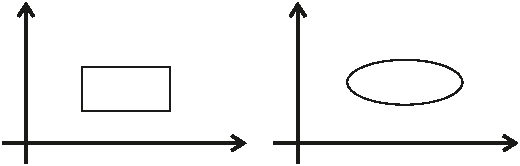
\includegraphics[width = 13cm]{pictures/picture_5_M.pdf}};
    \draw [color = black](-6.75,2.4) node[anchor = north west] { $\beta_0$ };
    \draw [color = black](0,2.4) node[anchor = north west] { $\beta_0$ };
    \draw [color = black](-1.2,-1.6) node[anchor = north west] { $\beta_1$ };
    \draw [color = black](5.45,-1.6) node[anchor = north west] { $\beta_1$ };
    \draw [color = black](2.9,0.25) node[anchor = north west] { $1 - \alpha$ };
    \draw [color = black](-3.9,0.2) node[anchor = north west] { $1 - \alpha$ };
    \end{tikzpicture}
\end{center}	
	
	 Zmíníme podrobněji u~vícerozměrné regrese.
\end{remark}


\subsection{TH pro~$\beta_0, \beta_1$ }

Chtěli bychom ověřit platnost předpokladu lineárního vztahu mezi~$x$ a~$y$.

Předpokládejme nyní, že model je lineární, a že $x$ je jediná dostupná vysvětlující proměnná. Otázkou zůstává, zda je $x$ užitečná ve~vysvětlení variability v~$y$, chceme tedy rozhodnout mezi~dvěma modely:
 $$
	Y_i = \beta_0 + e_i \quad \text{a} \quad Y_i = \beta_0 + \beta_1 x_i + e_i,
 $$
tzn. otestovat hypotézu $\hypothesis{\beta_1 = 0}{}\beta_1 \neq 0$.

Pokud nezamítneme $H_0$, závěr bude, že $x$ nevysvětluje nic z~variability $y$ a~není v~modelu významné. Pokud zamítneme $H_0$, znamená to, že $x$ je významné.

\begin{remark}
	Tyto závěry jsou správné pouze za~předpokladu, že model je lineární!
	\begin{itemize}
		\item Nezamítnutí $H_0$ nemusí znamenat, že $x$ není užitečná, může to pouze indikovat, že vztah mezi~$y$ a~$x$ není lineární.
		\item Zamítnutí $H_0$ naopak říká, že existuje lineární trend mezi~$x$ a~$y$, ale mohou tam být i~jiné typy závislostí.
	\end{itemize}
\end{remark}

Pro konstrukci testů využijeme odvozené IS.

\begin{remark}
	Opakování: $\hypothesis{\theta = \theta_0}{\theta \neq \theta_0} \Rightarrow (\underline{\theta}, \overline{\theta})$ je $100(1-\alpha)\%$ IS pro~$\theta$. Pak $W = \{ x | \theta_0 \notin (\underline{\theta}, \overline{\theta}) \}$ je kritický obor testu na~hladině $\alpha$.
\end{remark}

 $H_0: \beta_1 = 0$ zamítneme, pokud $0 \notin \left(\wbeta_1 \pm t_{1-\frac{\alpha}{2}}(n-2) \cdot  \frac{s_n}{\sqrt{\Sxx}} \right)$, tzn.
\begin{align*}
	\text{buď } \wbeta_1 + t_{1-\frac{\alpha}{2}}(n-2) \cdot  \frac{s_n}{\sqrt{\Sxx}} < 0 \quad\Leftrightarrow\quad \wbeta_1 \frac{\sqrt{\Sxx}}{s_n} < - t_{1-\frac{\alpha}{2}}(n-2) \\
	\text{nebo } \wbeta_1 - t_{1-\frac{\alpha}{2}}(n-2) \cdot  \frac{s_n}{\sqrt{\Sxx}} > 0 \quad\Leftrightarrow\quad \wbeta_1 \frac{\sqrt{\Sxx}}{s_n} > t_{1-\frac{\alpha}{2}}(n-2).
\end{align*}
A zapsáno dohromady
 $$
	|T_n| = |\wbeta_1| \frac{\sqrt{\Sxx}}{s_n} > t_{1-\frac{\alpha}{2}}(n-2).
 $$

\begin{remark}
	Intuitivní interpretace: $|T_n| = |\wbeta_1| \frac{\sqrt{\Sxx}}{s_n} = \frac{|\wbeta_1|}{\widehat{\sigma}(\wbeta_1)}$ je převrácená hodnota relativní chyby.
	
	Pokud je $\beta_1$ dobře odhadnuto, očekáváme malý rozptyl $\widehat{\sigma}(\wbeta_1)$, tedy $T$ bude velké.
	
	t-test tedy říká, že zamítneme $H_0$, pokud je relativní chyba odhadu malá.
\end{remark}% pages 21-30
\begin{remark}
	Někdy dopředu známe kandidáta $b_1$ jako hodnotu parametru $\beta_1$ a~chtěli bychom testovat
	 $\hypothesis{\beta_1 = b_1}{\beta_1\neq b_1}$. Test tedy zamítá $H_0$, pokud
	 $$ \abs{\beta_1-b_1}\cdot \frac{\sqrt{\Sxx}}{s_n}> t_{1-\frac{\alpha}{2}}(n-2). $$
\end{remark}
\subsubsection*{Test významnosti interceptu}
Otázka je, zda přímka prochází počátkem $(0,0)$, tedy $\hypothesis{\beta_0 = 0}{\beta_0\neq0}$. Nezamítnutí $H_0$ znamená, že jednodušší model $y = \beta_1 x+e$ lépe popisuje data, než $y = \beta_0+\beta_1 x+e$. $H_0$ potom zamítneme, pokud
 $$ T_n = \frac{|\widehat{\beta}_0|}{\widehat{\sigma}(\widehat{\beta}_0)} = |\widehat{\beta}_0|\frac{1}{s_n\sqrt{\frac{1}{n}+\frac{\overline{x}^2}{\Sxx}}}>t_{1-\frac{\alpha}{2}}(n-2). $$

\section{ANOVA přístup pro~testování}
Odvodili jsme t-test významnosti koeficientů a~nyní odvodíme ekvivalentní F-test, který může být zobecněn na~test celkové významnosti vícerozměrného regresního modelu (testy významnosti jednotlivých koeficientů mohou být totiž zavádějící).

Myšlenkou metody (analýza rozptylu ANOVA) je určit, kolik variability v~pozorováních $(y_1,y_2,...,y_n)$ je \uv{vysvětleno} regresním modelem (přímkou). Míru variability v~datech pak spočítáme jako podíl součtu sum od~regrese a~celkového počtu čtverců, tedy
 $$ \SST = \sumin(y_i-\overline{y}_n)^2, $$
pokud regresní přímka $y = \widehat{\beta}_0+\widehat{\beta}_1 x$ dobře prokládá data, tedy $\widehat{y}_i\approx y_i$. Dále bude platit, že
 $$ \sumin (\hyi-\lhyn)^2\approx\sumin (y_i-\lyn)^2. $$
Ukážeme, že $\lhy = \lyn$, a~tak
 $$ \sumin (\hyi-\lhyn)^2 = \sumin (\hyi-\lyn)^2 = \SSR, $$ což značí \textit{regression sum of squares} (regresní součet čtverců). Podíl
 $$ \RMR^2 = \frac{\SSR}{\SST} = \frac{\sumin (\hyi-\lyn)^2}{\sumin (y_i-\lyn)^2} $$ tak vyjadřuje podíl variability v~$(y_1,...,y_n)$ vysvětlené regresním modelem. Statistika $\RMR^2$ se nazývá \textbf{koeficient determinace} \textit{(coefficient of determination)} a pro každý model by měla mít hodnotu $\RMR^2\approx 1$.

Ukážeme, že $\RMR^2$ je kvadrát výběrového korelačního koeficientu mezi~$\textbf{x}$ a~$\textbf{y}$, což dává statistice $\RMR^2$ význam míry \uv{dobré shody}.

Pokud bychom znali rozdělení pravděpodobnostní statistiky $\RMR^2$, nabízí se~její použití pro~test $H_0:~\beta_1 = 0$, kterou bychom zamítli, pokud bude $\RMR^2\approx1$. Protože každá monotonní funkce $\RMR^2$ vede na~ekvivalentní test, budeme uvažovat statistiku 
\begin{equation}
	\NF = \frac{(n-2)\RMR^2}{1-\RMR^2}. \label{Definice F}
	\end{equation}

\begin{lemma}\label{lemma_k_vete}
	Nechť $\widehat{e}_i = y_i-\hyi$ značí rezidua, kde $\hyi = \wbeta_0+\wbeta_1 x_i$ a~$\wbeta_0,\wbeta_1$ jsou LSE. Potom \begin{enumerate}
		\item $\sumin \widehat{e}_i = 0$,
		\item $\lhyn = \lyn$,
		\item $\sumin \widehat{e}_i\hyi = 0$.
	\end{enumerate}
\begin{proof}
	\begin{enumerate}
		\item Z~rovnice $\frac{\partial S}{\partial\wbeta_0} = 0$ dostaneme $$ 0 = \sumin (y_i-\wbeta_0-\wbeta_1 x_i) = \sumin (y_i-\hyi) = \sumin \widehat{e}_i. $$
		\item Z~bodu 1) plyne, že $\sumin \hyi = \sumin y_i$, podělením $n$ dostaneme dokazované tvrzení.
		\item Z~rovnice $\frac{\partial S}{\partial\wbeta_1} = 0$ dostaneme $$ 0 = \sumin (y_i-\wbeta_0-\wbeta_1 x_i)x_i = \sumin \hei x_i, $$ a~tedy $$ \sumin \hei\hyi = \sumin \hei (\wbeta_0+\wbeta_1 x_i) = \sumin \hei\wbeta_0+\sumin x_i \hei\wbeta_1 = \wbeta_0\underbrace{\sumin \hei}_{ = 0}+\wbeta_1\underbrace{\sumin x_i\hei}_{ = 0} = 0. $$
	\end{enumerate}
\end{proof}
\end{lemma}
\begin{theorem}\label{vetasbysxx}
	Předpokládejme, že $\SST\neq 0$. Potom platí\begin{enumerate}
		\item $0\leq \RMR^2\leq1$,
		\item $\RMR^2 = 1-\frac{\SSE}{\SST}$, kde $\SSE = \sumin (y_i-\hyi)^2$ jako reziduální součet čtverců,
		\item $\RMR^2 = 1~\Leftrightarrow~(\forall i\in\widehat{n})(\hyi = y_i)$ (všechna data leží na~přímce),
		\item pokud označíme $\textbf{x} = (x_1,...,x_n)$ a~$\textbf{y} = (y_1,...,y_n)$, potom $\RMR^2 = \rho^2(\textbf{x},\textbf{y})$, kde $$ \rho(\textbf{x},\textbf{y}) = \frac{ \Big( \sumin (x_i-\overline{x}_n)(y_i-\lyn) \Big)^2}{\Sxx S_{yy}}, $$ tedy $\RMR^2$ je druhá mocnina výběrového korelačního koeficientu vektorů $\textbf{x},\textbf{y}$,
		\item $\NF = \frac{\SSR}{s_n^2} = \mathrm{T}^2$,
		\item pokud jsou chyby $e_1,...,e_n~iid~\NN(0,\sigma^2)$ a~$\beta_1 = 0$ (platí $H_0:~\beta_1 = 0$) v~modelu, potom $\NF\sim\NF(1,n-2)$.
	\end{enumerate}
\begin{proof}
	Důkaz věty bude založen na~rozkladu
	 $$ \sumin (y_i-\lyn)^2  = \sumin (\hyi-\ly)^2 + \sumin (y_i-\hyi)^2 \iff \SST = \SSR+\SSE.$$
	 Z~lemmatu \ref{lemma_k_vete} vyplývá, že
	\[
	\begin{split}
	\SST& = \sumin (y_i-\lyn)^2 = \sumin \left[(y_i-\hyi)+(\hyi-\lyn) \right]^2 = \\& = \sumin (y_i-\hyi)^2+\sumin (\hyi-\lyn)^2+2\sumin (y_i-\hyi)(\hyi-\lyn) = \SSE+\SSR+0,
	\end{split}
	\]
	neboť $$ \sumin \underbrace{(y_i-\hyi)}_{ = \hei}(\hyi-\lyn) = \underbrace{\sumin \hei\hyi}_{ = 0}-\lyn\underbrace{\sumin \hei}_{ = 0} = 0. $$
	Z toho potom dokazujeme jednotlivé body věty. \begin{enumerate}
		\item Protože $\SST = \SSE+\SSR$, pak $0\leq \RMR^2 = \frac{\SSR}{\SST}\leq \frac{\SST}{\SST} = 1$.
		\item $\SSR = \SST-\SSE~\Rightarrow~\RMR^2 = \frac{\SST-\SSE}{\SST} = 1-\frac{\SSE}{\SST}$.
		\item Z~bodu 2 plyne, že $\RMR^2 = 1~\Leftrightarrow~\SSE = 0$ a~$\SSE = \sumin (y_i-\hyi)^2 = 0~\Leftrightarrow~y_i = \hyi, ~\forall i\in\widehat{n}$.
		\item Platí $\hyi = \wbeta_0 + \wbeta_1 x_i = \lyn-\wbeta_1 \overline{x}_n + \wbeta_1 x_i = \lyn-\wbeta_1(\overline{x}_n-x_i)$. Proto pak
		$$ \SSR = \sumin (\hyi-\lyn)^2=\wbeta_1^2\sumin (x_i-\overline{x}_n)^2 = \wbeta_1^2 \Sxx, $$
		a~protože $\wbeta_1 = \frac{1}{\Sxx}\sumin (x_i-\overline{x}_n)(y_i-\lyn)$, dostaneme
		 $$ \rho^2(\textbf{x},\textbf{y}) = \frac{\Big[\sumin (x_i-\overline{x}_n)(y_i-\lyn)\Big]^2}{\Sxx S_{yy}} = \frac{\wbeta_1^2 \Sxx}{S_{yy}} = \frac{\SSR}{\SST} = \RMR^2, $$
		 neboť $S_{yy} = \sumin (y_i-\lyn)^2 = \SST$.
		\item Z~definice $\NF$ podle \eqref{Definice F} plyne, že
		 $$ \NF = \frac{(n-2)\RMR^2}{1-\RMR^2} = \frac{(n-2)\frac{\SSR}{\SST}}{\frac{\SSE}{\SST}} = \frac{\SSR}{\frac{\SSE}{n-2}} = \frac{\SSR}{s_n^2}. $$ Protože $\mathrm{T}_n = \wbeta_1\frac{\sqrt{\Sxx}}{s_n}$, pak $$ \mathrm{T}^2 = \frac{\wbeta_1^2 \Sxx}{s_n^2} = \frac{\SSR}{s_n^2} = F. $$
		\item $\mathrm{T}\sim t(n-2) \Rightarrow \NF = \mathrm{T}^2\sim\NF(1,n-2)$.
		
	\end{enumerate}
\end{proof}
\end{theorem}
\begin{remark}
\begin{enumerate}
	\item 	Z bodů 5 a~6 vyplývá, že použití libovolné statistiky $\mathrm{T}_n,\RMR^2$ nebo $\NF$ vede na~ekvivalentní test významnosti regrese.
	\item $\RMR^2$ poskytuje hrubou představu o~kvalitě modelu, čím je blíže $1$, tím lépe přímka prokládá data (nicméně je třeba jisté obezřetnosti, jak uvidíme později).
	\item $\NF$ lze chápat jako statistiku pro~test významnosti velkých hodnot $\RMR^2$.
\end{enumerate}
\end{remark}
Výsledky se~většinou uvádí v~tabulce ANOVA:
\begin{table}[h]\label{ANOVA_table}
	\begin{tabular}{|lllll|}
	\hline
	Source & df & SS & MS & $\NF$\\
	\hline
	Regression & 1 & $\SSR$ & MSR = $\SSR$ & $\frac{\mathrm{MSR}}{\mathrm{MSE}}$ \\
	Residual & $n-2$ & $\SSE$ & $\mathrm{MSE} = \frac{\mathrm{\SSE}}{n-2} = s_n^2$ & \\
	Total & $n-1$ & $\SST$ & & \\ \hline
\end{tabular}
\end{table}

Kde \textbf{Source} je zdroj součtu čtverců, \textbf{df} počet stupňů volnosti příslušný danému součtu čtverců, \textbf{SS} počet čtverců a~\textbf{MS} $(\mathrm{MS} = \frac{\mathrm{SS}}{\mathrm{df}})$ \uv{mean squares}.
\begin{remark}
	 $H_0:\beta_1 = 0$ je zamítnuta, pokud $\NF>\NF_{1-\alpha}(1,n-2)$. V~tomto jednorozměrném případě je to ekvivalentní t-testu, neboť $\NF = \mathrm{T}^2$.
\end{remark}
\begin{theorem}
	Mějme $e_1,...,e_n~iid~\NN(0,\sigma^2)$. Za~platnosti $H_0:~\beta_1 = 0$ je splněno, že
	 $$ \frac{\SSR}{\sigma^2}\sim\chi^2(1),\qquad\frac{\SSE}{\sigma^2}\sim\chi^2(n-2),\qquad\frac{\SST}{\sigma^2}\sim\chi^2(n-1). $$
\end{theorem}
\begin{remark}
	Proto se v~tabulce ANOVA \ref{ANOVA_table} uvádí df po~řadě $1,n-2,n-1$. Používají se~však i~v~případě jiného rozdělení chyb. Představit si je lze takto:
	\begin{enumerate}
		\item $\SSE = \sumin \hei^2$, na~$n$ reziduí $\he_1,...,\he_n$ máme 2 podmínky, $\sumin \hei = 0$ a~$\sumin x_i\hei = 0$. Z~toho vyplývá, že mají $n-2$ stupňů volnosti.
		\item $\SST = \sumin (y_i-\lyn)^2$, a proto musí $y_i-\lyn$ splňovat $\sumin (y_i-\lyn) = 0$, tudíž má $n-1$ stupňů volnosti.
		\item $\SSR = \SST-\SSE$ a~počet stupňů volnosti je roven $(n-1)-(n-2) = 1$.
	\end{enumerate}
\begin{proof}
	V důkazu věty \ref{vetasbysxx} jsme ukázali, že $\SSR = \wbeta_1^2 \Sxx$, takže $\frac{\SSR}{\sigma^2} = \left(\frac{\wbeta_1\sqrt{\Sxx}}{\sigma} \right)^2$. Víme, že $\wbeta_1\sim\NN\left(\beta_1,\frac{\sigma^2}{\Sxx}\right)$, a~tedy $(\wbeta_1-\beta_1)\frac{\Sxx}{\sigma}\sim\NN(0,1)$. Pro~$\beta_1 = 0$ tedy $$ \wbeta_1\frac{\sqrt{\Sxx}}{\sigma}\sim\NN(0,1)~\Rightarrow~\frac{\SSR}{\sigma^2}\sim\chi^2(1). $$
	Zároveň také $\frac{\SSE}{\sigma^2} = \frac{(n-2)s_n^2}{\sigma^2}\sim\chi^2(n-2)$ (viz tvrzení \ref{tvrzeni}) a~nezávisí na~$\wbeta_1$. Z~toho vyplývá, že $\frac{\SSR}{\sigma^2}$ a~$\frac{\SSE}{\sigma^2}$ jsou nezávislé. Dále platí, že
	 $$ \frac{\SST}{\sigma^2} = \frac{\SSR}{\sigma^2}+\frac{\SSE}{\sigma^2}~\Rightarrow~\frac{\SST}{\sigma^2}\sim\chi^2(n-1). $$
\end{proof}
\end{remark}
\begin{remark}
	 $\RMR^2$ statistika - pozor na~zjednodušení kvality modelu. \begin{enumerate}
		\item Nízké hodnoty $\RMR^2$ nemusí znamenat, že regresní model není významný. V~datech jen může být velké množství nevysvětlitelné náhodné variability. Například opakování hodnoty regresoru $x$ snižují hodnotu $\RMR^2$ oproti~modelům s~různými $x$.
		\item Velké hodnoty $\RMR^2$ mohou být způsobeny velkým měřítkem dat ($\Sxx$ je velká). Platí totiž, že
		 $$ \E(\RMR^2)\approx\frac{\beta_1^2 \Sxx}{\beta_1^2 \Sxx+\sigma^2}, $$ což je rostoucí funkce $\Sxx$.
		
		Velký rozptyl $(x_1,...,x_n)$ může mít za~následek velké $\RMR^2$ a~přitom nic neříká o~kvalitě modelu.
		
		 $\E(\RMR^2)$ je také rostoucí funkcí $\beta_1^2$. Modely s~velkou směrnicí tedy budou mít obecně větší $\RMR^2$, než modely s~\uv{malou} směrnicí.
	\end{enumerate}
\end{remark}

Při hodnocení kvality modelu potřebujeme více kritérií. Mezi~ně patří například\begin{enumerate}
	\item \uv{velké} $\RMR^2$,
	\item \uv{velké} $\NF$ nebo $|\mathrm{T}|$ hodnoty,
	\item \uv{malé} hodnoty $s_n^2$ vzhledem k~$\lyn$.
\end{enumerate}
Další kritéria budeme probírat později.
\begin{example}
	Velká hodnota $\RMR^2$ indikuje přibližně lineární vztah mezi~$x$ a~$y$, ale vysoký stupeň korelace nemusí znamenat příčinný vztah.
	Uveďme nyní říklad na datech z let 1924-1937. Mějme
	
	 $y_i$ - počet mentálních onemocnění na~$100000$ obyvatel Anglie.\\
	 $x_i$ - počet rádií v~populaci.\\
	Určíme parametry modelu $y_i = \beta_0+\beta_1 x_i+e_i$ jako
	 $$ \wbeta_0 = 4.5822,\qquad\wbeta_1 = 2.2042,\qquad\RMR^2 = 0.984, $$
	tzv. zjišťujeme velmi významný lineární vztah mezi~$x$ a~$y$. Závěr by mohl být, že rádia způsobují mentální onemocnění. I~když by to mohla být pravda, nabízí se~věrohodnější vysvětlení, a~to takové, že $x$ i~$y$ rostou lineárně s~časem, tzn. $y$ roste lineárně s~$x$.
	
	Rádia byla s~časem dostupnější, lepší diagnostické procedury umožňovaly identifikovat více lidí s~mentálními problémy.
\end{example}
\begin{remark}
Korelace VS příčinnost

 \begin{itemize}
  \item \textbf{Příčinná spojitost} -- i~když je příčinná spojitost mezi~$x$ a~$y$, korelace samotná nám neřekne, zda $x$ ovlivňuje $y$ nebo naopak.
  \item \textbf{Skrytá příčinnost} -- skrytá veličina $z$ ovlivňuje $x$ i~$y$, což způsobuje jejich korelovanost.
  \item \textbf{Confounding factor} -- skryté proměnné $z$ i~$x$ ovlivňují $y$, výsledek tedy závisí i~na~$z$.
  \item \textbf{Coincidence} -- korelace je náhodná.
\end{itemize}
\end{remark}

\section{Regrese skrz~počátek}
Existují případy, kdy přípustný model vyžaduje $\beta_0 = 0$, tj. $
 Y_i = \beta_1 x_i + e_i,~ i\in\widehat{n}$.


 \begin{enumerate}[1.]
  \item Na~základě fyzikálních úvah je předem známo, že
 $$
 \E [Y_0] = \beta_0 = 0.
 $$
		Potom tedy nemá smysl odhadovat $\beta_0$, protože to obecně sníží přesnost odhadu $\sigma^2$, a~tedy i~$\beta_1$.
  \item Na~začátek předpokládáme, že $\beta_0 \neq 0$ a~t-test nezamítne hypotézu $\text{H}_0 : \beta_0 = 0$, potom může být $\beta_0$ z~modelu odstraněn.
\end{enumerate}

\begin{remark}
V praktických situacích si často nemůžeme být jisti, že model platí i~blízko počátku. Část statistiků trvá na~přítomnosti interceptu v~modelu, i~když je nevýznamný.

Položit $\beta_0$ apriorně může být chybné, i~když $\E [Y_0] = 0$. Pokud totiž nevíme jistě, že model je lineární na~okolí 0, volba $\beta_0 = 0$ může vést k~vychýleným odhadům $\beta_1$, pokud jsou nezávislé proměnné daleko od~$x = 0$.
\end{remark}

\subsection{Odhady a~testy v~případě $\beta_0 = 0$ }
LSE parametr $\beta_1$ dostaneme minimalizací $S~ = \sumin (y_i - \beta_1 x_i)^2$ ve~tvaru
 $$
 \widehat{\beta}_1 = \frac{\sumin y_i  x_i }{\sumin x_i^2}.
 $$
Pokud $e_1,..., e_n~iid~\NN(0,\sigma^2)$, potom 
$$\E [\widehat{\beta}_1] = \beta_1\quad\text{a}\quad\D [\widehat{\beta}_1] = \frac{\sigma^2}{\sumin x_i^2}\quad\Rightarrow\quad\widehat{\beta}_1 \sim \NN\left(\beta_1, \frac{\sigma^2}{\sumin x_i^2}\right)$$
a $s_n^2 = \frac{1}{n-1}\sumin (y_i -  \widehat{y}_i)^2 = \frac{\SSE}{n-1}$ je nestranný odhad $\sigma^2$.
Dále $\frac{\SSE}{\sigma^2} \sim \chi^2(n-1)$ a~nezávisí na~$\widehat{\beta}_1$.
 $\text{H}_0 : \beta_1 = 0$ lze otestovat za~pomoci statistiky
 $$
  \mathrm{T} = \frac{\widehat{\beta}_1}{\frac{s_n}{\sqrt{\sum x_i^2}}} \sim \mathrm{t}(n-1),
 $$
kde $100(1-\alpha) \%$ IS pro~$\beta_1$ je $$\bigg(\widehat{\beta}_1 \pm \mathrm{t}_{1 - \frac{\alpha}{2}}(n-1)\frac{s_n}{\sqrt{\sum x_i^2}}\bigg).$$

Zatím je vše podobné jako pro~případ $\beta_1 \neq 0$. Rozdíl je ale v~tabulce ANOVA a~v~míře dobré shody. Problém je, že neplatí rozklad $\SST = \SSR + \SSE$, neboť součet reziduí $\sumin (y_i - \widehat{y})$ nemusí být 0, a~tedy $\overline{\widehat{y}}_n \neq \overline{y}_n$. Odvodíme nový rozklad, který platí v~obou případech, dokážeme ho ale jen pro~$\beta_0 = 0$.

\begin{theorem}
V modelu s~$\beta_0 = 0$ platí, že
 $$
 \sumin y_i^2 = \sumin \widehat{y}_i^2 + \sumin (y_i - \widehat{y}_i)^2.
 $$
\end{theorem}

\begin{proof}
 $$
 \sumin y_i^2 = \sumin (y_i - \widehat{y}_i + \widehat{y}_i)^2 = \sumin (y_i - \widehat{y}_i)^2 + \sumin \widehat{y}_i^2 + 2 \sumin (y_i - \widehat{y}_i) \widehat{y}_i
 $$
 Z rovnice $\frac{\d S}{\d \beta_1} = 0$ dostaneme $\sumin (y_i - \widehat{\beta}_1 x_i) x_i = 0
 $ a po vynásobení obou stran rovnic $\wbeta_1$ již máme
 $$
 \sumin (y_i - \widehat{y}_i) \widehat{y}_i = 0.
 $$
\end{proof}
Pokud vezmeme $\sum y_i^2$ jako míru variability v~datech, analogie $\RMR^2$ statistiky bude

 $$
  \RMR^2 = \frac{\sumin \widehat{y}_i^2}{\sumin y_i^2} \quad \Leftrightarrow \quad
  1 - \RMR^2 = \frac{\sumin y_i^2 - \sumin \widehat{y}_i^2}{\sumin y_i^2} = \frac{\sumin \widehat{e}_i^2}{\sumin y_i^2 }
 $$
Definujeme $F : = \frac{(n-1) \RMR^2}{1 - \RMR^2}$. Potom
 $$
  F = \frac{\sumin \widehat{y}_i^2 }{\frac{1}{n-1} \sumin (y_i - \widehat{y}_i)^2 } = \frac{\widehat{\beta}_1 \sumin x_i^2 }{ s_n^2} = \text{T}^2.
 $$
Vztah mezi~$\RMR^2, \NF$ a $\mathrm{T}^2$ je tedy stejný jako pro~$\beta_0 \neq 0$.

\begin{remark}
  Tato definice $\RMR^2$ se~ale v~praxi moc nepoužívá, protože neumožňuje přímé srovnání modelů s~interceptem a bez něj.
\end{remark}
 $$
  \beta_0 = 0  : \quad \RMR^2 = 1 - \frac{\SSE}{\sumin y_i^2},
\qquad
  \beta_0 \neq 0  : \quad \RMR^2 = 1 - \frac{\SSE}{\sumin (y_i - \oynn)^2}.
 $$

Obecně ale $\sumin (y_i - \oynn)^2 < \sumin y_i^2$, $\RMR^2$ v~modelu s~$\beta_0 = 0$ tedy bude větší, než $\RMR^2$ modelu s~$\beta_0 \neq 0$, i~když jsou jejich $\SSE$ srovnatelné.

\begin{enumerate}[1.]
  \item Definice vhodné $\RMR^2$ pro~$\beta_0 = 0$ vyvolává jistou kontroverzi a~existuje několik verzí.
  \item Možná volba je $\RMR^2 = \left(\rho (y_I, \overline{y}_I)\right)^2$, kde $\overline{y}_I = (\overline{y}_1,...,\overline{y}_n)$, protože tato vlastnost platí i~pro~případ $\beta_0 = 0$.
  \item Další možnost je srovnat modely pomocí hodnot $s_n^2$ (preferujeme~model s~nejnižší hodnotou $s_n^2$).
\end{enumerate}\begin{table}[h]
	\begin{tabular}{lllll}
		Source & df & SS & MS & F \\
		\hline
		Regression & $1$ & $\SSR = \sumin \hyi^2$ & MSR $ = \frac{\SSR}{1}$ & $\frac{\SSR}{s_n^2}$ \\
		Residual & $n-1$ & $\SSE = \sumin (y_i = \hyi)^2$ & MSE $ = \frac{\SSE}{n-1}$ &  \\
		Total & $n$ & $\SST = \sumin y_i^2$ &  &  \\
		\hline
		&  & $\RMR^2 = \rho^2(\textbf{y},\widehat{\textbf{y}})$ &  &  \\
	\end{tabular}
\caption{Tabulka ANOVA pro~$\beta_0 = 0$.}
\end{table}

\section{Predikce}
Jakmile máme model, často bývá cílem odhadnout hodnoty veličiny $Y_0$ pro~nové $x_0$, které není v~původních datech. Budeme uvažovat dva typy predikce:\begin{enumerate}[1)]
	\item predikce střední hodnoty $\mu_0 = \EE{Y_0}$ v~bodě $x_0$,
	\item predikce hodnoty nového pozorování $Y_0$ v~bodě $x_0$.
\end{enumerate}
Pro oba typy použijeme bodový odhad
 $ \widehat{Y}_0 = \wbeta_0+\wbeta_1 x_0. $
Intervalové odhady se~ale budou lišit.

\subsection*{Ad 1)}
	Protože je $\mu_0 = \beta_0+\beta_1 x_0$ vlastně parametr, lze pro~něj odvodit IS (za předpokladu normality chyb).
	Spočteme tedy $\D(\widehat{Y}_0)$. Dosazením odhadů $\wbeta_0$ a~$\wbeta_1$ dostaneme $\widehat{Y}_0 = \overline{y}+\wbeta_1(x_0-\overline{x})$ a
	 $$ \D\widehat{Y}_0 = \D(\overline{Y})+(x_0-\overline{x})^2\D(\wbeta_1)+2(x_0-\overline{x})\underbrace{\Cov(\overline{Y},\wbeta_1)}_{ = 0} = \frac{\sigma^2}{n}+\frac{\sigma^2(x_0-\overline{x})^2}{\Sxx} = \sigma^2\left[\frac{1}{n}+\frac{(x_0-\overline{x})^2}{\Sxx} \right]. $$
	
	Nahrazením $\sigma^2$ statistikou $s_n^2$ dostaneme odhad $\D(\widehat{Y}_0)$ ve~tvaru
	 $$ \widehat{\sigma}^2(\widehat{Y}_0) = s_n^2\left[\frac{1}{n}+\frac{(x_0-\lx)^2}{\Sxx} \right]. $$
	 $\wsigma(\hY_0)$ se~obvykle nazývá \textbf{standardní chyba predikce v~bodě $x_0$ }. Jsou-li $e_1,...,e_m~iid~\NN(0,\sigma^2)$, platí, že
	 $$ \hY_0\sim\NN\bigg(\mu_0,\underbrace{\sigma^2\left[\frac{1}{n} + \frac{(x_0-\lx)^2}{\Sxx} \right]}_{\sigma^2(\hY_0)} \bigg), $$a~tedy
	 $$ \frac{\hY_0-\mu_0}{\sigma(\hY_0)}\sim\NN(0,1). $$
	Celkově tedy dostáváme
	 $$ T = \frac{\frac{\hY_0-\mu_0}{\sqrt{\sigma^2\left(\frac{1}{n}+\frac{(x_0-\lx)^2}{\Sxx}\right)}}}{\sqrt{\frac{(n-2)s_n^2}{\sigma^2}\frac{1}{n-2}}} = \frac{\hY_0-\mu_0}{\sqrt{s_n^2\left(\frac{1}{n}+\frac{(x_0-\lx)^2}{\Sxx} \right)}} = \frac{\hY_0-\mu_0}{\wsigma(\hY_0)}\sim t(n-2). $$
	
	Vyjádřením získáme $100(1-\alpha)$ \% IS pro~$\mu_0$ ve~tvaru $$ \hY_0\pm t_{1-\frac{\alpha}{2}}(n-2)\wsigma(\hY_0). $$
	\begin{remark}
		Z tvaru IS je vidět, že bude nejkratší pro~$x_0 = \lx$ a~s~rostoucí vzdáleností $| x_0-\lx |$ se~prodlužuje.\begin{itemize}
			\item  Speciálně potom čím dále jsme od~oblasti, kde jsou naše data $x$, tím méně spolehlivé jsou naše predikce.
			\item Je třeba opatrnosti při~predikci hodnot $Y$ mimo interval $(\min x_i,\max x_i)$.
		\end{itemize}
\end{remark}

\subsection*{Ad 2)}
Intervalové odhady pro~$Y_0$ nejsou IS, protože $Y_0$ není parametr. Říká se~jim \textbf{intervaly predikce}. Potřebujeme znát hodnotu rozptylu $Y_0-\hY_0$. Pokud je pozorování $Y_0$ nezávislé na~$Y_i,~i\in\widehat{n}$, potom
 $$ \D(Y_0-\hY_0) = \underbrace{\D Y_0}_{\sigma^2}+\D \hY_0+0 = \sigma^2\left[1+\frac{1}{n}+\frac{(x_0-\lx)^2}{\Sxx} \right]. $$ Odhad tohoto rozptylu bude $s_p^2$, kde
 $$ s_p = s_n\sqrt{1+\frac{1}{n}+\frac{(x_0-\lx)^2}{\Sxx}}. $$

Za předpokladu normality chyb pak
 $$ T = \frac{Y_0-\hY_0}{s_n\sqrt{1+\frac{1}{n}+\frac{(x_0-\lx)^2}{\Sxx}}} = \frac{Y_0-\hY_0}{s_p}\sim t(n-2). $$
Vyjádřením získáme $100(1-\alpha)$ \% interval predikce pro~$Y_0$ ve~tvaru
 $$ \hY_0 \pm t_{1-\frac{\alpha}{2}}(n-2)s_p. $$

\begin{remark}
	Přesnost predikce \begin{enumerate}[a)]
		\item roste s~rostoucím $n$ a~rostoucím rozsahem $x$ naměřeným pomocí $\Sxx$,
		\item klesá s~rostoucím $|x_0-\lx|$.
	\end{enumerate}
Pokud můžeme předem zvolit $x_1,..., x_n$, lze přesnost predikce zvýšit volbou dostatečně rozptýlených hodnot $x$. To ale může zvyšovat $\RMR^2$ a~někdy vést k~horšímu modelu.

To je \textbf{základní rozpor v~regresní analýze}:
\begin{itemize}
	\item dobrý model nemusí poskytovat dobré predikce,
	\item dobré predikce mohou vycházet z~méně přesných modelů.
\end{itemize}
\end{remark}
\begin{remark}
	Odvozené výsledky platí za~předpokladu normality chyb. Protože jsou ale za~podmínek regularity odhady $\wbeta_0,\wbeta_1$ asymptoticky normální, IS pro~$\EE{Y_0}$ budou fungovat (jsou použitelné i~pro~velká $n$). IP pro~$Y_0$ ale závisí na~normalitě  chyb i~pro~velká $n$, mohou tedy být nepřesné pro~nenormální chyby.
\end{remark}
\begin{example}[Ověření adekvátnosti modelu]Ověření adekvátnosti modelu je důležitá součást analýzy. Měla by být provedena dříve, než budeme interpretovat parametry modelu nebo přijímat nějaké závěry založené na~modelu.
	
	Všechny výsledky týkající se~$\beta_0,\beta_1$ byly odvozeny za~předpokladu \textbf{linearity modelu} a~některé za~předpokladu \textbf{normality chyb}.
	Bylo by tedy dobré mít testy ověřující linearitu.
	
\section{Základní procedury pro ověření linearity}
\begin{enumerate}[1)]
	\item Prozkoumání \textbf{scatter plotu} dvojic $(x_i,y_i)$. Příklad lze vidět na~obrázku \ref{SCATTER}. Takový scatter plot může indikovat, že lepší model bude
	 $$ y_i = \beta_0+\beta_1 x_i+\beta_2 x_i^2+e_i. $$
	\begin{figure}[h]
		\centering
		\begin{tikzpicture}[line cap = round,line join = round,> = triangle 45,x = 1.0cm,y = 1.0cm]
		\draw[->,color = black] (-0.62,0) -- (3.88,0);
		\foreach \x in {,2}
		\draw[shift = {(\x,0)},color = black] (0pt,-2pt);
		\draw[->,color = black] (0,-0.68) -- (0,2.8);
		\clip(-0.62,-0.68) rectangle (3.88,2.8);
		\draw [color = black](2.7,-0.15) node[anchor = north west] { $x_i$ };
		\draw [color = black](-0.6,2) node[anchor = north west] { $y_i$ };
		\begin{scriptsize}
		\fill [color = black] (0.52,0.48) circle (1.5pt);
		\fill [color = black] (1.16,0.6) circle (1.5pt);
		\fill [color = black] (1.8,0.9) circle (1.5pt);
		\fill [color = black] (2.22,1.3) circle (1.5pt);
		\fill [color = black] (2.54,1.76) circle (1.5pt);
		\fill [color = black] (2.8,2.24) circle (1.5pt);
		\end{scriptsize}
		\end{tikzpicture}
		\caption{Scatter plot naměřených dat.}
		\label{SCATTER}
	\end{figure}
	Scatter plot ale může být zavádějící, pokud je odklon od~linearity způsoben spíše chybějící proměnnou, než polynomiální závislostí na~$x$.
	\item \textbf{Analýza hodnot testovacích statistik.}
	\begin{itemize}
		\item Např. malá hodnota $\RMR^2$ společně s~významnou hodnotou t-statistiky pro~parametry $\beta_1$ obecně naznačuje, že skutečný model obsahuje i~jiné proměnné $x$,
		\item velká hodnota $\RMR^2$ a~významná t-statistika ale samo o~sobě neznamená, že je model lineární.
	\end{itemize}
\item \textbf{Obrázky reziduí}. Je to efektivní diagnostický nástroj. Rezidua odhadují, kolik variability v~datech zůstane po~odstranění lineární části v~$x$. Dá se~také očekávat, že jejich hodnoty budou užitečné pro~detekci odchylek od~normality.

	
\end{enumerate}	
	
\end{example}
\begin{example}
	Analýza scatter plotů a~obrázků reziduí je dost subjektivní. Bylo by dobré mít nějaký objektivní analytický nástroj pro~ověření linearity modelu. Bohužel nejsou k~dispozici skoro žádné takové nástroje. Pro~většinu dat jsou v~praxi nejvíce využívány metody 1) - 3).
	
	Jinak je tomu u~navržených experimentů typu industriálních nebo klinických studií, kde existuje doporučený analytický test, tzv. \textit{lack of fit} test (LOFT). Ten předpokládá, že máme více pozorování pro~jednu $x_i$.
\end{example}

\subsection*{Ad 3) - Analýza reziduí}
Intuitivně, pokud je náš model správný, měla by se~rezidua chovat jako náhodný výběr z~$\NN(0,\sigma^2)$. Pokud se~bude zdát, že se~tak nechovají, bude to znamenat neadekvátnost modelu. Později ukážeme grafický nástroj. Nejprve ale začneme vlastnostmi reziduí.

\begin{theorem}
	Nechť $\hei$ jsou rezidua modelu \eqref{Model 1D LR} odhadnutého metodou nejmenších čtverců. Potom platí, že
	\begin{enumerate}
		\item $\E \hei = 0, \quad i\in\widehat{n} $,
		\item $\D \hei = \sigma_{\hei}^2 = \sigma^2 \left[1 - \left(\frac{1}{n} + \frac{(x_i - \hx)^2}{\Sxx} \right) \right] \approx \sigma^2$ pro~velká $n$,
		\item $\Cov (\hei, \hej) = -\sigma^2 \left[1 - \left(\frac{1}{n} + \frac{(\hx - x_i)(\hx - x_j)}{\Sxx} \right) \right]$,
		\item $\Cov(\hei, \hYi) = 0, \quad i\in\widehat{n} $.
		\item Pokud jsou $e_1,..., e_n$~iid~$\Nn$, potom platí, že
		 $$
			\hZi = \frac{\hei}{\sigma_{\hei}} \sim \NN (0,1).
		 $$
	\end{enumerate}
\end{theorem}

\begin{proof}
\begin{enumerate}
	\item $\hei = Y_i - \hYi$, takže $\E(\hei) = \E Y_i - \E \hYi$, ale $\E \hYi = \E(\model) = \beta_0 + \beta_1 x_i = \E Y_i$.
	\item
	 $$
		\D \hei = \D (Y_i - \hYi) = \D Y_i + \underbrace{\D \hYi}_{\sigma^2 \left[\frac{1}{n} + \frac{(x_i - \hx)^2}{\Sxx} \right]} - 2 \underbrace{\Cov(Y_i, \hYi)}_{\sigma^2 \left[\frac{1}{n} + \frac{(x_i - \hx)^2}{\Sxx} \right]} = \sigma^2 \left[1 - \left(\frac{1}{n} + \frac{(x_i - \hx)^2}{\Sxx} \right) \right].
	 $$
	\item
	\begin{align*}
		\Cov(\hei, \hej) & = \Cov(Y_i - \hYi, Y_j - \hYj) = \underbrace{\Cov(Y_i, Y_j)}_{ = 0} - \Cov(Y_i, \hYj) - \Cov(Y_i, \hYj) + \Cov(\hYi, \hYj), \\
		\Cov(\hYi, \hYj) & = \Cov(\model, \wbeta_0 + x_j \wbeta_1) = \underbrace{\D(\wbeta_0)}_{\sigma^2 \left[\frac{1}{n} + \frac{\hx^2}{\Sxx} \right]} + (x_i + x_j) \underbrace{\Cov (\wbeta_0,\wbeta_1)}_{-\frac{\sigma^2 \hx}{\Sxx}} + x_i x_j \underbrace{\D(\wbeta_1)}_{\frac{\sigma^2}{\Sxx}} = \\
		& = \sigma^2 \left[\frac{1}{n} + \frac{\hx^2}{\Sxx} - \frac{(x_i + x_j) \hx}{\Sxx} + \frac{x_i x_j}{\Sxx}\right] = \sigma^2 \left[\frac{1}{n} + \frac{(x_i - \hx)(x_j - \hx)}{\Sxx} \right].
	\end{align*}
	
	Podobně bychom dostali
	 $$
		\Cov(Y_i, \hYj) + \Cov(\hYi, Y_j) = 2 \sigma^2 \left[\frac{1}{n} + \frac{(x_i - \hx)(x_j - \hx)}{\Sxx} \right],
	 $$
	takže $\Cov(\hei, \hej) = - \sigma^2 \left[\frac{1}{n} + \frac{(x_i - \hx)(x_j - \hx)}{\Sxx} \right]$.
	\item
	 $$
		\Cov(\hei, \hYi) = \Cov(Y_i - \hYi, \hYi) = \underbrace{\Cov(Y_i, \hYi)}_{ = \sigma^2 \left[\frac{1}{n} + \frac{(x_i - \hx)^2}{\Sxx} \right]} - \underbrace{\D(\hYi)}_{ = \Cov(\hYi, \hYi) = \sigma^2 \left[\frac{1}{n} + \frac{(x_i - \hx)^2}{\Sxx} \right]} = 0.
	 $$
	\item $e_i \sim \Nn \Rightarrow \hei \sim \NN(\cdot, \cdot)$, protože $\hei$ je LK $Y_1,..., Y_n$
	\begin{align*}
		\text{1)} & \Rightarrow \E \hei = 0 \\
		\text{2)} & \Rightarrow \D \hei = \sigma_{\hei}^2 \\
	 			  & \Rightarrow \frac{\hei}{\sigma_{\hei}} \sim \NN(0,1)
	\end{align*}
	\end{enumerate}
\end{proof}

\begin{remark}
	Z bodu 3) věty plyne, že $\Cov(\hei, \hej) \approx 0$ pro~velké $n$. Pokud jsou testy $e_i$~iid~$\Nn$, měla by se~standardizovaná rezidua $\hZi = \frac{\hei}{\sigma_{\hei}}$ chovat pro~velké $n$ jako náhodný výběr z~$\NN(0,1)$ rozdělení. V~praxi ale budeme potřebovat odhad $\sigma^2$ pro~výpočet $\hZi$.
	
	Nejznámější procedura je proto odhadnout $\sigma^2$ pomocí $s_n^2$. Potom by se~měla \textbf{standardizovaná rezidua}
	 $$
		\hzi := \frac{\hei}{s_n \sqrt{1 - \left(\frac{1}{n} + \frac{(x_i - \hx)^2}{\Sxx} \right)}}
	 $$
	pro~velká $n$ opět chovat jako náhodná veličina z~$\NN(0,1)$.
\end{remark}

\begin{remark}
	 $\hei$ se~užívají pro~grafickou analýzu.
	
	Existuje ale i jiná třída reziduí, tzv. PRESS rezidua.
	
	Označme $\wbeta_{0(-i)}, \wbeta_{1(-i)}$ odhady parametrů $\beta_0, \beta_1$, pokud je vynecháno i-té pozorování. Pak i-té PRESS reziduum je definováno jako
	 $$
		\widehat{e}_{(-i)} = \hYi - \widehat{Y}_{(-i)}, \quad \text{kde \;} \widehat{Y}_{(-i)} = \wbeta_{0(-i)} + x_i \wbeta_{1(-i)}.
	 $$
	Podrobněji se~jim budeme věnovat později.
\end{remark}

\section{Grafy reziduí}
\begin{itemize}
	\item \underline{Histogram reziduí} -- umožní náhled normality reziduí.
	\item \underline{Kvantilový graf (QQ plot) standardizovaných reziduí} -- seřadíme dle velikosti: $\hr_{(1)} \leq \hr_{(2)} \leq... \leq \hr_n$ a~vyneseme oproti~$\Phi^{-1}\left((i - \frac{1}{2}) \frac{1}{n} \right)$, $i  \in\widehat{n} $. Body by měly ležet přibližně na~přímce ($\E (e_i) \approx \Phi^{-1}\left((i - \frac{1}{2}) \frac{1}{n} \right)$ pro~normální chyby).
	
	Použití: ověření normality, detekce odlehlých pozorování (obr. 3.6 str. 1077 GLM).
	\item \underline{Standardizovaná rezidua $\times$ jednotlivým vysvětlujícím proměnným $x$} -- $\hr_i$ nezávisí na~$\sigma$, graf $\hr_i \times x_i$ lze použít pro~detekci nelinearity nebo nekonstantního rozptylu.
	\item \underline{Standardizovaná rezidua $\hr_i \times$ predikovaným hodnotám $\hyi$} -- $\Cov(\hei, \hYi) = 0$, tedy $\hei(\hr_i)$ a~$\hYi$ by měly být nekorelované, pokud platí model \eqref{Model 1D LR}. To znamená, že graf $\hr_i \times \hyi$ by měl být náhodně rozptýlený kolem~osy $x$, navíc $\hr_i$ by měla ležet v~$(-3,3)$ ($ \hr_i \approx \NN(0,1) $).
	(doplnit obrázky)
	\item \underline{Standardizovaná rezidua $\times$ pořadí pozorování} -- možná detekce řadové korelace mezi~pozorováními.
	(doplnit obrázky)
	
\end{itemize}

